% Title page
\frame[plain]{\titlepage}

% Lesson 1. Introduction, main terms and simple examples
\lecture{Intro}{intro}

\section{Tools}

\begin{frame}
	\frametitle{\insertsection}
	We are going to use SWI-Prolog~--- a comprehensive free Prolog environment.
	\begin{itemize}
		\item You can download SWI-Prolog at this page: \href{https://www.swi-prolog.org/download/stable}{https://www.swi-prolog.org/download/stable}
		\item Complete manual is available at \href{https://www.swi-prolog.org/pldoc/doc_for?object=manual}{https://www.swi-prolog.org/pldoc/doc\_for?object=manual}
		\item Online tool SWISH: \href{https://swish.swi-prolog.org/}{https://swish.swi-prolog.org/}
		\item Eclipse PDT~--- Prolog Development Tool
	\end{itemize}
\end{frame}

\section{Overview}

\begin{frame}
	\frametitle{\insertsection}
	Goals of the lesson
	\begin{itemize}
		\item Look into the syntax of Prolog language
		\item Define the main terms of Prolog: fact, rule, query, and knowledge base
		\item Define basic syntax units, such as atom, variables and term
		\item Look at some example programs and try to figure out what they do
		\item Get out feet wet with some programming
	\end{itemize}
\end{frame}

\section{Basic constructs}

\begin{frame}
	\frametitle{\insertsection}
	Basic Prolog constructs
	\begin{tabular}{p{0.4\textwidth}p{.6\textwidth}}
		\begin{itemize}
			\item \textbf{Facts}. Facts are used to state things that are unconditionally true in the domain of interest.
			\item \textbf{Rules}. Rules state information that is conditionally true of the domain of interest.
		\end{itemize}
		&
		\begin{itemize}
			\item[] \textbf{Knowledge Base} (also called database) is a collection of facts and rules. Prolog programs are knowledge
			bases, collections of facts and rules which describe some collection of relationships that we find interesting. We use knowledge base
			by posing queries.
		\end{itemize}
	\end{tabular}
	\begin{itemize}
		\item \textbf{Queries}. The Prolog interpreter responds to queries about the facts and rules represented in its database. In making a query you are asking Prolog whether it can prove that your query is true. If so, it answers "Yes" and displays any \textit{variable bindings} that it made in coming up with the answer. If it fails to prove the query true, it answers "No".
	\end{itemize}
\end{frame}

\section{Simple Examples}

\begin{frame}
	\frametitle{\insertsection}
	\textbf{Example 1}: Simple knowledge base
	
	\begin{tabular}{p{0.4\textwidth}|l}
			\textbf{Knowledge base} & \only<2->{\textbf{Possible queries and responses}} \\
			\hline
			\hline
			\texttt{
				\begin{tabular}{p{0.5\textwidth}}
					fruit(orange).\\
					fruit(apple).\\
					vegetable(potato).\\
					vegetable(onion).\\
					\only<3->{common(you).\\
						uncommon(chuck\_norris).\\
						makes\_cry(onion, Person) :- common(Person).\\
						makes\_cry(Person, onion) :- uncommon(Person).\\
					}
				\end{tabular}
			} &
			\texttt{\only<2>{\begin{tabular}{l l}
				?- fruit(orange). & \textbf{true.} \\
				\hline
				?- fruit(onion). & \textbf{false.} \\
				\hline
				?- fruit(tomato). & \textbf{false.} \\
				\hline
				?- berry(watermelon). & \textbf{ERROR}
			\end{tabular}} \only<4->{\begin{tabular}{p{0.3\textwidth}p{0.2\textwidth}}
				?- makes\_cry(chuck\_norris, onion). & \textbf{true.} \\
				\hline
				?- makes\_cry(onion, you). & \textbf{true.} \\
				\hline
				?- makes\_cry(you, onion). & \textbf{false.} \\
				\hline
				?- makes\_cry(Who, Whom). & Who=you, \newline  Whom=onion; \newline  Who=chuck\_norris, \newline  Whom=onion. \\
		\end{tabular}}}
	\end{tabular}
\end{frame}

\begin{frame}
	\frametitle{\insertsection}
	\textbf{Example 2}: Conjunctions and disjunctions in rules
	
	\begin{tabular}{p{0.5\textwidth}|l}
		\textbf{Knowledge base} & \only<2->{\textbf{Possible queries and responses}} \\
		\hline
		\hline
		\texttt{
			\begin{tabular}{p{0.5\textwidth}}
				lovesMusic(anna).\\
				lovesMusic(sam).\\
				playsInstrument(anna).\\
				musician(P) :- lovesMusic(P),\newline playsInstrument(P).\\
				melomaniac(P) :- !,lovesMusic(P);\newline playsInstrument(P).\\
			\end{tabular}
		} &
		\texttt{\only<2->{\begin{tabular}{p{0.3\textwidth}p{0.2\textwidth}}
					?- musician(anna) & \textbf{true.} \\
					\hline
					?- musician(sam) & \textbf{false.} \\
					\hline
					?- melomaniac(anna) & \textbf{true.} \\
					\hline
					?- melomaniac(sam) & \textbf{true.} \\
					\hline
					?- melomaniac(Person) & \textbf{Person=sam; Person=anna.}
			\end{tabular}}}
	\end{tabular}
\end{frame}

\begin{frame}
	\frametitle{\insertsection}
	\textbf{Example 3}: Negations
	
	\begin{tabular}{p{0.5\textwidth}|l}
		\textbf{Knowledge base} & \only<2->{\textbf{Possible queries and responses}} \\
		\hline
		\hline
		\texttt{
			\begin{tabular}{p{0.5\textwidth}}
				cat(fluffy).\\
				cat(cornie).\\
				bird(butch).\\
				dog(bayley).\\
				good(fluffy).\\
				hasClaws(X) :- cat(X).\\
				hasClaws(X) :- bird(X).\\
				hasClaws(X) :- not(dog(X)).\\
				animal(X) :- cat(X);bird(X);dog(X).\\
				domestic(X) :- animal(X),not(hasClaws(X)).\\
				domestic(X) :- animal(X),good(X).\\
			\end{tabular}
		} &
		\texttt{\only<2->{\begin{tabular}{p{0.3\textwidth}p{0.2\textwidth}}
					?- domestic(bayley). & \textbf{true.} \\
					\hline
					?- domestic(cornie). & \textbf{false.} \\
					\hline
					?- cat(C),domestic(C) & \textbf{C = fluffy.}\\
					\hline
					?- cat(C),not(domestic(C)) & \textbf{C = cornie.}
		\end{tabular}}}
	\end{tabular}
\end{frame}

\section{Prolog Syntax}

\begin{frame}
	\frametitle{\insertsection}
	\textbf{Facts, rules and queries in Prolog are built of terms}
	\begin{itemize}
		\item Atoms
		\item Numbers
		\item Strings
		\item Variables
		\item Compex terms~--- structures
	\end{itemize}
\end{frame}

\begin{frame}
	\frametitle{\insertsection}
	\textbf{Atoms}
	\begin{enumerate}
		\item A string of characters made up of upper-case letters, lower-case letters, digits, and underscore characters,
		that begins with a lower-case letter.
		\item An arbitrary sequence of characters enclosed in single quotes.
		\item A sequence of special characters.
	\end{enumerate}

	\begin{example}
		\texttt{chuck\_norris, bayley, cornie, someCamelCaseStringNumber1, 'Chuck Norris', 'Some arbitrary string', '@!?@',
		=====>, :-, @>}
	\end{example}
\end{frame}

\begin{frame}
	\frametitle{\insertsection}
	\textbf{Numbers}
	\begin{enumerate}
		\item \textbf{Real numbers}, though not particularly important in typical applications, are supported in Prolog.
		\item[] \begin{example}
			2.71828, 82.19284, \(\pi, e \), \ldots
		\end{example}
		\item \textbf{Integers} are useful for many tasks, such as counting the elements of a list.
		\item[] \begin{example}
			\(-2, -1, 0, 1, 2, 3, \ldots \)
		\end{example}
	\end{enumerate}
\end{frame}

\begin{frame}
	\frametitle{\insertsection}
	\textbf{Variables and strings}
	\begin{enumerate}
		\item A variable is a sequence of upper-case letters, lower-case letters, digits and underscore character
		that starts either with an upper-case letter or with underscore.
		\item[] \begin{example}
			\texttt{X, Y, Var, Chuck\_Norris, \_someVar, \_1zx, \_}
		\end{example}
		\item String is an arbitrary sequence of characters enclosed in double quotes.
		\item[] \begin{example}
			"Some arbitrary string line"
		\end{example}
	\end{enumerate}
\end{frame}

\begin{frame}
	\frametitle{\insertsection}
	\textbf{Complex terms}
	\only<1>{\begin{itemize}
		\item Complex terms are built out of \textbf{functor (predicate)} followed by a sequence of \textbf{arguments}.
		\item The arguments are put in parentheses and are separated by commas.
		\item The functor of a term \textbf{must} be an atom.
		\item Arguments can be any kind of term.
		\item The number of arguments that a complex term has is called its \textbf{arity}.
	\end{itemize}}
	\only<2->{\begin{itemize}
			\item Any \textbf{constant} is a term. Constants are atoms, numbers or strings.
			\item Any \textbf{variable} is a term.
			\item Any sequence of a form \texttt{f(a1, a2, \ldots)} where \texttt{f} is an atom, and
			\texttt{a1, a2,}~\ldots are terms, is a term.
			\item There are no other terms.
	\end{itemize}
	\begin{example}
		\texttt{g(f(x, y))}
	\end{example}}
	
\end{frame}

\begin{frame}
	\frametitle{\insertsection}
	Which of the character sequences are atoms, variables or neither of them?
	\texttt{\begin{enumerate}
		\item vARIABLE
		\item Variable
		\item x
		\item XY1
		\item chuck\_norris\_tells\_simon\_what\_to\_do
		\item \_john
		\item '\_jonh'
		\item 'John likes everybody'
		\item Chuck Norris plays russian roulette with a fully loded revolver and wins
	\end{enumerate}}
\end{frame}

\begin{frame}
	\frametitle{\insertsection}
	Which of the sequences are terms, and which are not. For every term indicate its functor and arity.
	\texttt{\begin{enumerate}
		\item loves(vincent,mia)
		\item 'loves(vincent,mia)'
		\item Eats(cat,mouse)
		\item hasChildren(cat,kittens)
		\item and(musician(jody),artist(mia))
		\item and(musician(X),artist(Y))
		\item \_and(musician(jody),artist(mia))
		\item (Butch kills Vincent)
		\item kills(Butch,Vincent)
	\end{enumerate}}
\end{frame}

\begin{frame}
	\frametitle{\insertsection}
	How many facts, rules, clauses and predicates there are in the knowledge base?
	
	\texttt{
		\begin{tabular}{l}
			cat(fluffy).\\
			cat(cornie).\\
			bird(butch).\\
			dog(bayley).\\
			good(fluffy).\\
			hasClaws(X) :- cat(X).\\
			hasClaws(X) :- bird(X).\\
			hasClaws(X) :- not(dog(X)).\\
			animal(X) :- cat(X);bird(X);dog(X).\\
			domestic(X) :- animal(X),not(hasClaws(X)).\\
			domestic(X) :- animal(X),good(X).\\
		\end{tabular}
	}
\end{frame}

\section{Exercise}

\begin{frame}
	\frametitle{\insertsection}
	\textbf{Write the following statements in Prolog}
	
	\texttt{\begin{tabular}{l}
			1. Any giraffe is a horse that was uppercutted by Chuck Norris \\
			2. Mia and Marcellus are married \\
			3. Zed is dead \\
			4. If something is on fire then it smokes \\
			5. Marsellus kills everyone who gives Mia a footmassage \\
			6. Mother of a mother is a grandmother \\
			7. Mia loves everyone who is a good dancer
	\end{tabular}}
\end{frame}


% Lesson 2. Term matching.
\lecture{Match}{match}
%\setcounter{framenumber}{1}

\section{Overview}

\begin{frame}
	\frametitle{\insertsection}
	Goals of the lesson
	\begin{itemize}
		\item Discuss the idea of matching in Prolog.
		\item Explain the differences between Prolog matching and standard unification.
		\item Introduce the built-in predicate for matching.
		\item Explain the search strategy Prolog uses when trying to prove something.
	\end{itemize}
\end{frame}

\section{Matching}

\begin{frame}
	\frametitle{\insertsection}
	\begin{itemize}
		\item The basic idea of matching is follows: \textbf{Two terms match, if they are equal or if they contain variables that can be
			instantiated in such a way that the resulting terms are equal}.
		\item The built-in binary predicate \texttt{=/2} tests whether its two arguments match.
	\end{itemize}
	
	\textbf{The following terms match:}
	
	\texttt{
		\begin{tabular}{l}
			orange = orange. \\
			fruit(orange) = fruit(orange). \\
			cat(C) = cat(fluffy). \\
			cat(C) = cat(cornie). \\
			f(g(X,Y)) = f(g(x, Z)). \\
			f(g(X,Y)) = f(g(Z,y)). \\
			f(g(X,Y)) = f(g(a,b)).
		\end{tabular}
	}
\end{frame}

\begin{frame}
	\frametitle{\insertsection}
	\begin{enumerate}
		\item If \texttt{term1} and \texttt{term2} are constants, then \texttt{term1} and \texttt{term2} match if and only if they are the same atom, the same string or the same number.
		\item If \texttt{term1} is a variable and \texttt{term2} is any type of term, then \texttt{term1} and \texttt{term2} match, and \texttt{term1} is instantiated to \texttt{term2}. Vice versa is also true. If they are both variables, they’re both instantiated to each other, and we say that they \textbf{share values}.
		\item If \texttt{term1} and \texttt{term2} are complex terms, then they match if and only if:
		\begin{enumerate}
			\item They have the same functor and arity.
			\item All their corresponding arguments match.
			\item The variable instantiations are compatible.
		\end{enumerate}
		\item Two terms match if and only if it follows from the previous three clauses that they match.
	\end{enumerate}
\end{frame}

\begin{frame}
	\frametitle{\insertsection}
	\textbf{Let us have some examples:}
	
	\texttt{
		\begin{tabular}{p{0.8\textwidth} | l}
			chuckNorris = chuckNorris. & \textbf{true.} \\
			\hline
			100 = 100. & \textbf{true.} \\
			\hline
			chuckNorris = "chuckNorris". & \textbf{false.} \\
			\hline
			chuckNorris = 'chuckNorris'. & \textbf{true.} \\
			\hline
			100 = '100' & \textbf{false.} \\
			\hline
			Var1 = Var2 & \textbf{true.} \\
			\hline
			triang(p(1,1),p(Px,Py),p(Px1,8)) = triang(P,p(7,4),p(n(7),8)). & \textbf{true.} \\
			\hline
			triang(p(X,X),p(2,5),p(7,11)) = triang(p(1,7), P2, P3). & \textbf{false.} \\
			\hline
			f(X) = X. & \textbf{true?}
		\end{tabular}
	}
\end{frame}

\section{Unification}

\begin{frame}
	\frametitle{\insertsection}
	\begin{itemize}
		\item Terms are symbolic expressions used to model logical propositions.
		\item Terms can easily be represented as trees, where variables and constants are leaves and functors are branches.
		\item A substitution of terms is a set of variables paired with terms: \(\left\{(x_1\rightarrow t_1 ),\ldots, (x_n\rightarrow t_n ) \right\} \), where each pair represents a variable \(x_i\), that should be substituted with a term \(t_i\).
		\item \textbf{Unification} is the process of unifying equations, called terms, so that they become equivalent. This is done by finding a substitution which when applied on the variables of the terms will result in them becoming identical.
		\item A unification algorithm commonly takes 2 terms and returns this substitution if it exists. The substitution that unifies the terms is called \textbf{a unifier}.
	\end{itemize}
\end{frame}

\begin{frame}
	\frametitle{\insertsection}
	\begin{itemize}
		\item A unification algorithm performs \textbf{the occur check}.
		\item The occur check checks whether a variable appears among the arguments of the functor, which it is being unified with. This is required to prohibit infinite terms like \(X = f(X)\), which results in something like \(f(f(f(f(\ldots)))) \). This can create cycles that could cause termination problems.
	\end{itemize}

	Suppose we have the following terms. What will the Standard Unification Algorithm do?
	
	\begin{table}
		\centering
		\begin{tabular}{c}
			\(f(X_1, X_2, \ldots, X_n) \) \\
			\\
			\(f(g(X_0, X_0), g(X_1, X_1), \ldots, g(X_{n-1}, X_{n-1}) \)
		\end{tabular}
	\end{table}
\end{frame}

\begin{frame}
	\frametitle{\insertsection}
	\begin{table}
		\centering
		\begin{tabular}{c}
			\(f(X_1, X_2, \ldots, X_n) \) \\
			\\
			\(f(g(X_0, X_0), g(X_1, X_1), \ldots, g(X_{n-1}, X_{n-1}) \)
		\end{tabular}
	\end{table}
	\only<1>{
		\begin{itemize}
			\item Obviously enough, the algorithm will reduce the problem by recognizing that the two functors are identical.
			\item Then problem becomes to transform the variable input of the two functors such that they become identical. Hence the algorithm will start unifying the variables of \(f\).
			\item First \(X_1\) will be substituted with \(g(X_0, X_0)\). The rest of the list will then replace each instance of \(X_1\) with \(g(X_0, X_0)\).
			\item The latter means that \(X_2\) will be substituted with \(g(g(X_0, X_0), g(X_0, X_0)\) and so on.
		\end{itemize}
	}
	\only<2->{
		\begin{tabular}{l}
			\(X_1\rightarrow g(X_0, X_0) \) \\ \\
			\(X_2\rightarrow g(g(X_0, X_0), g(X_0, X_0)) \) \\ \\
			\(X_3\rightarrow g(g(g(X_0, X_0), g(X_0, X_0)), g(g(X_0, X_0), g(X_0, X_0)))  \) \\ \\
			\vdots \\ \\
			\(X_n\rightarrow g(g(g(g(g\ldots  \)
		\end{tabular}
	}
\end{frame}

\begin{frame}
	\frametitle{\insertsection}
	\begin{itemize}
		\item Prolog \textbf{omits} the occur check when matching terms since the running time of the occur check can escalate.
		\item Standard unification algorithms are \textbf{pessimistic}. They first look	for strange variables (using the occurs check) and only when they are sure that the two terms are "safe" do they go ahead and try and match them. So a standard unification algorithm will never get locked into a situation where it is endlessly trying to match two unmatchable terms.
		\item Prolog, on the other hand, is \textbf{optimistic}. It assumes that you are not going to give it anything dangerous. So it does not make an occurs check. As soon as you give it two terms, it charges full steam ahead and tries to match them.
	\end{itemize}
\end{frame}

\section{Proof search}

\begin{frame}
	\frametitle{\insertsection}
	Suppose we are working with the following knowledge base:
	
	\begin{tabular}{p{0.52\textwidth}|l}
		\texttt{
			\begin{tabular}{p{0.5\textwidth}}
				verb(drinks).\\
				noun(milk).\\
				noun(cat).\\
				article(a).\\
				subj(cat).\\
				obj(milk).\\ \\
				phrase(A,S,V,O) :- article(A), noun(S), subj(S), verb(V), noun(O), obj(O).\\ \\
			\end{tabular}
		} &
		\texttt{{
			\begin{tabular}{p{0.4\textwidth}}
				Suppose we then pose a query: \textbf{phrase(A,S,V,O).} \\ \\
				The answer will be \\ \\
				A = a, \\ S = cat, \\ V = drinks, \\ O = milk
			\end{tabular}
		}}
	\end{tabular}
\end{frame}

\begin{frame}
	\frametitle{\insertsection}
	\begin{figure}
		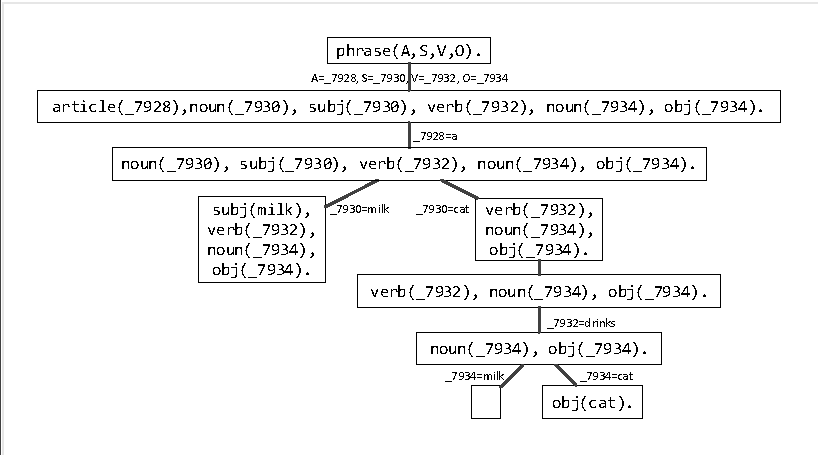
\includegraphics{prooftree}
	\end{figure}
\end{frame}

\section{Exercise}

\begin{frame}
	\frametitle{\insertsection}
	Which of the following pairs of terms match? Where relevant, give the variable instantiations that lead to successful matching.
	\texttt{\begin{enumerate}
		\item a = a, 'String' = string, x = Y.
		\item f(X, Y, z) = f(x, a, b).
		\item g(x, y, f(Z)) = g(Z, Y, f(x)).
		\item polygon(v(x1,y1), v(x1,Y), v(X,Y)) = polygon(v(X,Z), v(x1,y2), v(x3,y3)).
		\item polygon(v(x1,y3), v(x2,Y), v(X,Y)) = polygon(v(X,Y), v(Z,y3), v(x1,y3)).
		\item move(state(Pos,onTheFloor,Pos,H), push(Pos,Pos1), state(Pos1,onTheFloor,Pos1,H)) = move(state(x,onTheFloor,Pos,no), push(x,y), state(Pos1,onTheFloor,Pos1,no)).
	\end{enumerate}}
\end{frame}


% Lesson 3. Recursion in Prolog
\lecture{Recursion}{recursion}

\section{Overview}

\begin{frame}
	\frametitle{\insertsection}
	Goals of the lesson
	\begin{itemize}
		\item Introduce recursive definitions in Prolog
		\item Discuss the mismatches between the declarative meaning of a Prolog program, and its procedural meaning
	\end{itemize}
\end{frame}


\section{Recursive definitions}

\begin{frame}
	\frametitle{\insertsection}
	Predicates can be defined recursively. It means that one or more rules in predicate's definition refers to itself.
	
	\only<1>{The most common example is a description of family relationships.}
	\only<2>{\textbf{Basis}}
	\only<3->{\textbf{Step}}
	
	\texttt{
		\begin{tabular}{l}
			{\color<2>[RGB]{255,0,0}{ancestor(Anc,Dec) :- child(Dec,Anc).}} \\
			{\color<3->[RGB]{255,0,0}{ancestor(Anc,Dec) :- child(Dec,Par), ancestor(Anc,Par).}} \\
			child(jane, peter). \\
			child(mary, kate). \\
			child(sam, mary). \\
			child(jason, jane). \\
			child(ann, jason).
		\end{tabular}
	}
\end{frame}


\begin{frame}
	\frametitle{\insertsection}
	
	Next, let us define natural numbers, having a definition of zero and a rule of succession. This representation is variously called successor arithmetic, successor notation and also \textbf{Peano arithmetic}.
	
	\texttt{
		\begin{tabular}{l}
			num(0). \\
			num(s(N)) :- num(N). \\ \\
			\uncover<2->{sum(0, N, N). \\
				sum(s(M), N, s(S)) :- sum(M, N, S).
			}
		\end{tabular}
	}

	\uncover<3->{Our numbers will be something like: \(0, s(0), s(s(0)), s(s(s(0))), \ldots\) Not very pleasant if you want to compute something, but sometimes used
	in automated provers.}
	
\end{frame}


\section{Tail recursion}

\begin{frame}
	\frametitle{\insertsection}
	
	Suppose we want to compute factorial (in normal numbers this time). We already know about recursion, and after a while will end up with a program similar to this one:
	
	\texttt{
		\begin{tabular}{l}
			f(0,1). \\
			f(N,F) :- N > 0, M is N - 1, f(M,Acc), F is Acc*N.
		\end{tabular}
	}

	Binary predicate \texttt{f/2} takes two arguments: natural number N and factorial of N. The table below shows possible queries.
	
	\texttt{\begin{table}\centering\begin{tabular}{l | l}
			f(4, F). & F = 24. \\
			\hline
			f(5, 120). & true. \\
			\hline
			f(X, 120). & ERROR \\
	\end{tabular}\end{table}}	
	
\end{frame}


\begin{frame}
	\frametitle{\insertsection}
	
	A recursive function is \textbf{tail recursive} when recursive call is the last thing executed by the function. It works in Prolog just well.
	Let us rewrite our factorial function, and make it tail recursive.
	
	\texttt{
		\begin{tabular}{l}
			f(N,N,F,F) :- !. \\
			f(N,M,Acc,F) :- M1 is M + 1, Acc1 is Acc * M1, f(N,M1,Acc1,F). \\
			factorial(N,F) :- f(N,1,1,F).
		\end{tabular}
	}

	As we can see predicate \texttt{f} takes 4 arguments now: natural number N, computation step M, result computed on step M, and total result F. Below are some examples.
	
	\texttt{\begin{table}\centering\begin{tabular}{l | l}
				factorial(4, F). & F = 24. \\
				\hline
				factorial(5, 120). & true. \\
				\hline
				factorial(X, 120). & X = 5. \\
	\end{tabular}\end{table}}	
	
\end{frame}


\section{Clause ordering, goal ordering, and termination}

\begin{frame}
	\frametitle{\insertsection}
	
	\only<1>{Recall our family program which as we know works just fine:}
	\only<2->{But what happens if we swap goals in the second rule?}
	
	\texttt{
		\begin{tabular}{l}
			ancestor(Anc,Dec) :- child(Dec,Anc). \\
			\only<1>{ancestor(Anc,Dec) :- child(Dec,Par), ancestor(Anc,Par).}
			\only<2->{\underline{ancestor(Anc,Dec) :- ancestor(Anc,Par), child(Dec,Par).}}\\
			child(jane, peter). \\
			child(mary, kate). \\
			child(sam, mary). \\
			child(jason, jane). \\
			child(ann, jason).
		\end{tabular}
	}

	\uncover<2->{If we pose query \texttt{ancestor(jane, ann)} we will get a correct answer (\texttt{true}), and then an error message which means that Prolog is looping. }

\end{frame}

\begin{frame}
	\frametitle{\insertsection}
	\begin{figure}
		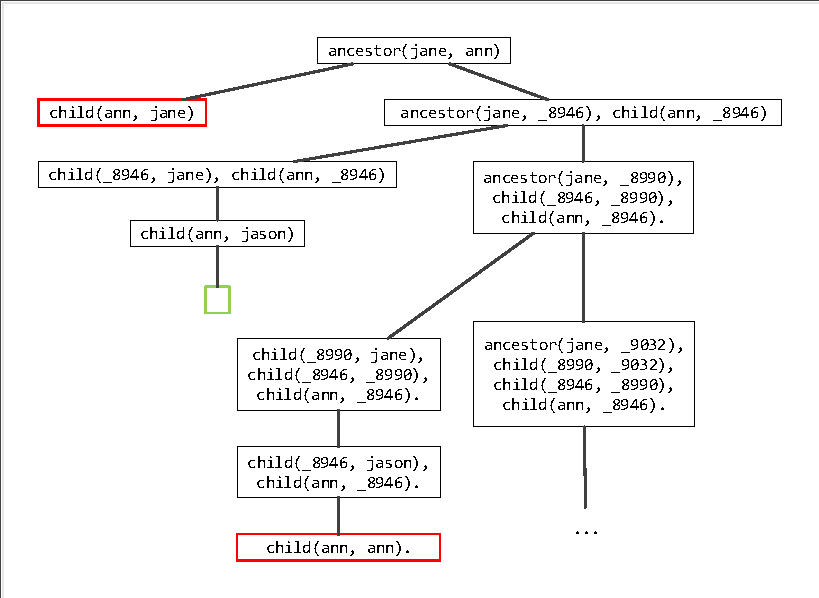
\includegraphics[scale=0.78]{badtree}
	\end{figure}
\end{frame}


% Lesson 5 Arithmetic in Prolog
\lecture{Arithmetic}{arithmetic}


\section{Overview}

\begin{frame}
	\frametitle{\insertsection}
	Goals of the lesson
	\begin{itemize}
		\item To introduce Prolog’s inbuilt abilities for performing arithmetic.
		\item To discuss how they can be applied to other data types' processing problems.
	\end{itemize}
\end{frame}


\section{Drawbacks of the successor arithmetic}

\begin{frame}
	\frametitle{\insertsection}
	
	Recall our Peano arithmetic implementation.
	
	\texttt{
		\begin{tabular}{l}
			num(0). \\
			num(s(N)) :- num(N).
		\end{tabular}
	}

	This is a pure predicate that terminates if any of the arguments is instantiated. We can read the clauses declaratively to reason about the cases that this relation describes. Other elementary relations between natural numbers can be defined analogously.
\end{frame}


\begin{frame}[shrink=4]
	\frametitle{\insertsection}
	
	Unfortunately, this representation of natural numbers suffers from several significant disadvantages:
	\begin{itemize}
		\item First, this is not really the way we want to write and read numbers. We would like to use a more familiar notation~--- such as 1, 2 and 3—to represent natural numbers.
		\item With some practice, we may get used to the successor notation. However, a more fundamental problem remains: This representation takes space that is directly proportional to the magnitude of the numbers we need to represent. Thus, the space requirement grows exponentially with the length of any number's decimal representation. Therefore, reasoning about larger numbers is infeasible with this representation.
		\item More complex relations such as multiplication and exponentiation are hard to define in such a way that they work in all directions and retain good termination properties.
		\item To extend this representation to integers, we also need a way to represent negative numbers.
	\end{itemize}
	
\end{frame}


\begin{frame}
	\frametitle{\insertsection}
	\justifying
	Therefore, successor notation~—-- albeit useful to illustrate different ways in which we could represent our data~—-- is not how we typically reason about numbers in Prolog.
\end{frame}


\begin{frame}
	\frametitle{\insertsection}
	\justifying
	Instead, we use built-in predicates to reason about numbers in Prolog. In the case of integers, these predicates are known as \textbf{CLP(FD)} constraints, and in more recent systems also as CLP(\(\mathds{Z} \)) constraints. CLP(FD) stands for \textbf{Constraint Logic Programming over Finite Domains} and reminds us of the fact that in reality, we can only represent a finite subset of integers on actual machines, while \(\mathds{Z} \) denotes the integers and indicates that these constraints are designed for reasoning about all integers.
	
	All widely used Prolog implementations provide CLP(FD) constraints. However, the exact details differ slightly between various systems. For example, in GNU Prolog, B-Prolog and other systems, CLP(FD) constraints are conveniently available right from the start. In contrast, you need to load a library to use them in SICStus Prolog and other systems.
	
	SWI Prolog provides a number of basic arithmetic tools for manipulating integers.
\end{frame}


\section{Arithmetic in Prolog}

\begin{frame}[shrink=3]
	\frametitle{\insertsection}
	
	SWI-Prolog defines the following numeric types:
	
	\begin{itemize}
		\item \textbf{Integer} If SWI-Prolog is built using the GNU multiple precision arithmetic library (GMP), integer arithmetic is unbounded, which means that the size of integers is limited by available memory only. Without GMP, SWI-Prolog integers are 64-bits, regardless of the native integer size of the platform. The inbuild predicate \texttt{integer/1} holds if
		an argument is an integer.
		\item \textbf{Rational number} Rational numbers (\(\mathds{Q} \)) are quotients of two integers (\(\frac{N}{M} \)). Rational arithmetic is only provided if GMP is used. Rational numbers satisfy the type tests \texttt{rational/1}, \texttt{number/1} and \texttt{atomic/1} and may satisfy the type test \texttt{integer/1}, i.e., integers are considered rational numbers. Rational numbers are always kept in canonical representation, which means \(M\) is positive and \(N\) and \(M\) have no common divisors.
		\item \textbf{Float} Floating point numbers are represented using the C type double. On most of today's platforms these are 64-bit IEEE floating point numbers. Satisfy the type tests \texttt{float/1}, \texttt{number/1} and \texttt{atomic/1}.
	\end{itemize}

\end{frame}


\begin{frame}
	\frametitle{\insertsection}
	
	\begin{table}
		\centering
		\begin{tabular}{ l | r }
			\rowcolor{Gray}
			\textbf{Arithmetic expression} & \textbf{Same in Prolog} \\
			\hline
			\rowcolor{LightGray}\( 10 + 5 = 15 \) & \texttt{15 is 10 + 5.}   \\
			\rowcolor{LightGray}\( 10\cdot 5 = 50 \)  & \texttt{50 is 10 * 5.}   \\
			\rowcolor{LightGray}\( 10 - 5 = 5 \)  & \texttt{5 is 10 - 5.}   \\
			\rowcolor{LightGray}\( 5 - 10 = -5 \)  & \texttt{-5 is 5 - 10.}   \\
			\rowcolor{LightGray}\( 10~/~5 = 2 \)  & \texttt{2 is 10 / 5.}   \\
			\rowcolor{LightGray}\( 10~/~4 = 2.5 \)  & \texttt{2.5 is 10 / 4.}   \\
			\rowcolor{LightGray}\( 10~/~4 = 4\cdot 2 + 2 \)  & \texttt{2 is mod(10,4).}  \\
		\end{tabular}
	\end{table}
	
\end{frame}


\begin{frame}
	\frametitle{\insertsection}
	
	\begin{table}
		\centering
		\begin{tabular}{ l | r }
			\rowcolor{Gray}
			\textbf{Arithmetic expression}   & \textbf{Same in Prolog} \\
			\hline
			\rowcolor{LightGray}\( x < y \) & \texttt{X < Y.}  \\
			\rowcolor{LightGray}\( x\leqslant y \)  & \texttt{X =< Y.}   \\
			\rowcolor{LightGray}\( x = y \)  & \texttt{X =:= Y.}  \\
			\rowcolor{LightGray}\( x\neq y \)  & \texttt{X =\= Y.}  \\
			\rowcolor{LightGray}\( x\geqslant y \)  & \texttt{X >= Y.}  \\
			\rowcolor{LightGray}\( x > y \)  & \texttt{X > Y.} \\
		\end{tabular}
	\end{table}
	
\end{frame}


\begin{frame}
	\frametitle{\insertsection}
	
	SWI-Prolog provides many extensions to the set of floating point functions defined by the ISO standard.
	
	\begin{example}
		\texttt{sin, cos, tan, log, log10, exp, **, sqrt, ceil, floor, round, abs, max, min, >>, <<}
	\end{example}
\end{frame}


\begin{frame}
	\frametitle{\insertsection}
	
	Normally all Prolog does is just unification of variables to structures. Arithmetic is something extra that has been bolted on to the basic Prolog engine because it is useful.
	
	Arithmetic functions are terms which are evaluated by the arithmetic predicates. Apart from the fact that the functors go between their	arguments instead of in front of them these are ordinary Prolog terms, and unless we	do something special, Prolog will not actually do any arithmetic.
	
	To force Prolog to actually evaluate arithmetic	expressions we have to use inbuild binary predicate \texttt{is/2}.
	
\end{frame}


\begin{frame}
	\frametitle{\insertsection}
	
	Since arithmetic functions is an extra stuff in Prolog then it is not surprising that there are some restrictions on this extra ability.
	
	\begin{itemize}
		\item The arithmetic expressions to be evaluated must be on the right hand side of \texttt{is}.
		\item Moreover, every variable on the right hand side must already have been instantiated to a number. If the variable is uninstantiated, or if it is instantiated to something
		other than a number, we will get some sort of \texttt{instantiation\_error} message.
	\end{itemize}

\end{frame}


\begin{frame}
	\frametitle{\insertsection}
	
	Here’s an example.
	
	\texttt{double(N, D) :- D is N * 2.}
	
	This predicate simply doubles its first argument and returns the answer in its second argument.
	
	\begin{itemize}
		\item \texttt{double(5, A)} returns \texttt{A = 10.}
		\item But posing the query \texttt{double(Half, 10)} does not return anything. Instead we get the \texttt{instantiation\_error} message. When we pose the query, we are asking Prolog
		to evaluate expression \texttt{10 is Half * 2}, which is impossible due to uninstantiation of \texttt{Half}.
	\end{itemize}
	
	\begin{example}
		\texttt{15 is 10 + 5.} \(\Leftrightarrow \) \texttt{is(15,+(10,5)).} \\
		\texttt{X is (2*5 + 10) / 4.} \(\Leftrightarrow \) \texttt{is(X,/(+(*(2,5),10),4)).}
	\end{example}
\end{frame}


% Lesson 6. Lists
\lecture{Lists}{lists}


\section{Overview}

\begin{frame}
	\frametitle{\insertsection}
	Goals of the lesson
	\begin{itemize}
		\item To introduce lists, an important recursive data structure widely used in computational linguistics.
		\item To define predicates Prolog provides to work with lists.
		\item To introduce the idea of recursing down lists.
	\end{itemize}
\end{frame}


\section{Functional notation}

\begin{frame}
	\frametitle{\insertsection}
	
	Lists are Prolog terms for which there are dedicated syntactic provisions.
	
	Lists are defined inductively:
	
	\begin{itemize}
		\item The atom \texttt{[]} (nil) is a list. It denotes an empty list.
		\item The compound term \texttt{.(H, T)} is a list iff \texttt{T} is a list. \texttt{H} is a first element or \textbf{head} of the list, and \texttt{T} is a \textbf{tail} of the list.
	\end{itemize}

	As if to make canonical definition of lists more painful in SWI Prolog predicate \texttt{'[|]'} is used instead of \texttt{'.'}.
\end{frame}

\begin{frame}
	\frametitle{\insertsection}
	
	\begin{table}
		\begin{center}
			\begin{tabular}{m{5cm} c}
				\only<1>{
					\texttt{[]}
					&
					An empty list
				}
				\only<2>{
					\texttt{'[|]'(a,[])}
					& 
					\begin{tabular}{c}
						\raisebox{-\totalheight}{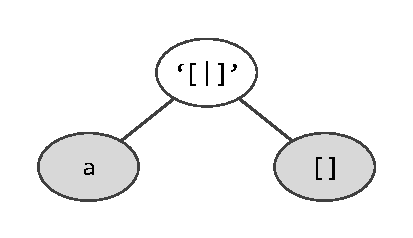
\includegraphics[scale=1.3]{list1}}
					\end{tabular}
				}
				\only<3>{
					\texttt{'[|]'(a, '[|]'(b, []))}
					&
					\begin{tabular}{c}
						\raisebox{-\totalheight}{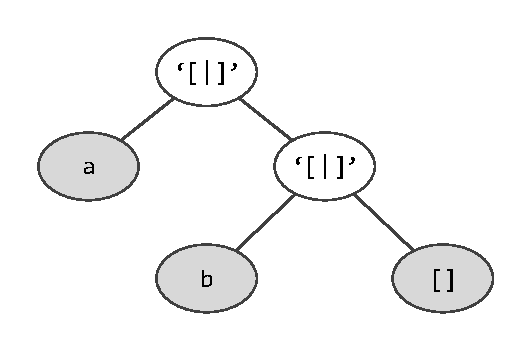
\includegraphics{list2}}
					\end{tabular}
				}
			\end{tabular}
		\end{center}
	\end{table}
\end{frame}


\section{List notation}

\begin{frame}
	\frametitle{\insertsection}
	
	\begin{itemize}
		\item List is a finite sequence of elements.
		\item Lists in Prolog are specified by enclosing the elements in square brackets [...].
		\item The elements are separated by commas: \texttt{[one, two, three, 1, 2]}. The length of a list is a number of its elements. Any term could be an element of a list.
		\item Any non-empty list can be thought of as consisting of the head and the tail. The head is simply the first item in the list; the tail is everything else. SWI Prolog has a special inbuilt operator | which can be used to decompose a list into its head and tail.
		\item The empty list contains no internal structure.
	\end{itemize}
\end{frame}


\begin{frame}
	\frametitle{\insertsection}
	
	\begin{table}
		\begin{center}
			\begin{tabular}{m{3cm} c}
				\only<1>{
					\texttt{[]}
					&
					An empty list
				}
				\only<2>{
					\texttt{[a]}
					& 
					\begin{tabular}{c}
						\raisebox{-\totalheight}{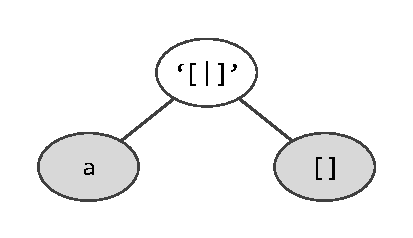
\includegraphics[scale=1.3]{list1}}
					\end{tabular}
				}
				\only<3>{
					\texttt{[a, b]}
					&
					\begin{tabular}{c}
						\raisebox{-\totalheight}{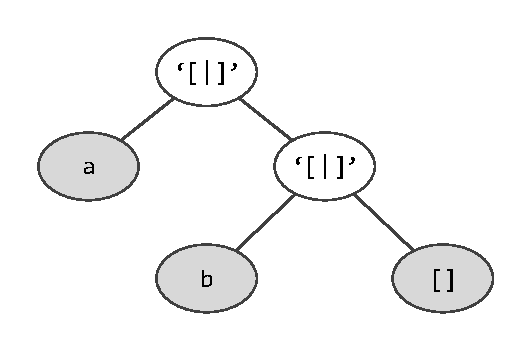
\includegraphics{list2}}
					\end{tabular}
				}
				\only<4>{
					\texttt{[a, b, c]}
					&
					\begin{tabular}{c}
						\raisebox{-\totalheight}{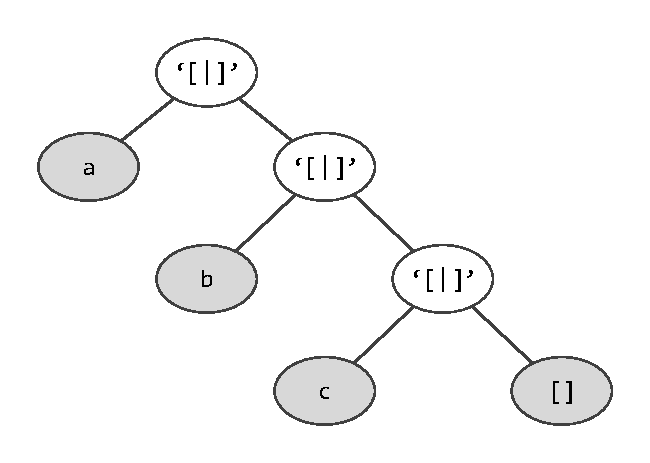
\includegraphics[scale=0.88]{list3}}
					\end{tabular}
				}
			\end{tabular}
		\end{center}
	\end{table}
\end{frame}


\begin{frame}
	\frametitle{\insertsection}
	
	\texttt{\begin{itemize}
			\item[] []
			\item[] [first, second, third, fourth, fifth]
			\item[] [1, 2, 3, 4, 5, 6, 7, 8, 9, 0]
			\item[] [first, 2, color(cornie, black), F, fifth, F]
			\item[] [first, second, [third, fourth], [fifth, color(cornie, black)]]
			\item[] [[], [], car(volkswagen), F, 1, 2, [1, F, car(bmw), [1, 2, 4]], X]
	\end{itemize}}
\end{frame}


\section{Elements and operations}

\begin{frame}
	\frametitle{\insertsection}
	
	\texttt{\begin{itemize}
			\item[] [abyssian, bobtail, [bengal, birman]]
	\end{itemize}}
	
	\texttt{\begin{itemize}
			\item<2-> {[H|T]} = [abyssian, bobtail, [bengal, birman]].
			\item<3-> {[F,S|T]} = [abyssian, bobtail, [bengal, birman]].
			\item<4-> {[\_,S|T]} = [abyssian, bobtail, [bengal, birman]].
			\item<5-> {[First,\_,\_,Fourth|\_]} = [abyssian, bobtail, [bengal, birman]].
			\item<6-> {[\_,\_,[\_|T]|\_]} = [abyssian, bobtail, [bengal, birman]].
	\end{itemize}}
	
\end{frame}


\begin{frame}
	\frametitle{\insertsection}
	
	The inbuilt predicate \texttt{member/2 = member(?Elem, ?List)} is True if \texttt{Elem} is a member of \texttt{List}, and False otherwise.
	
	\texttt{\begin{table}\centering\begin{tabular}{l | l}
		member(a, []). & false. \\
		\hline
		member(a, [b, a, 1, [], f(a, b, c)]) & true
	\end{tabular}\end{table}}

	\texttt{\begin{itemize}
			\item<2->[] member(X, [X|T]).
			\item<3->[] member(X, [H|T]) :- member(X,T).
	\end{itemize}}
	
	\uncover<4->{\texttt{\begin{itemize}
				\item[] member(X, [X|\_]).
				\item[] member(X, [\_|T]) :- member(X,T).
	\end{itemize}}}
\end{frame}


\begin{frame}
	\frametitle{\insertsection}
	
	Other operations on lists:
	
	\begin{enumerate}
		\item Length of a list.
		\item Concatenation.
		\item Prefix, suffix and a sublist of a list.
		\item Get last element.
		\item List reversal.
		\item Sorting.
	\end{enumerate}
\end{frame}


% Lesson 7 Definite Clause Grammars
\lecture{DCG}{dcg}


\section{Overview}

\begin{frame}
	\frametitle{\insertsection}
	Goals of the lesson
	\begin{itemize}
		\item To introduce context free grammars (CFGs) and some related concepts.
		\item To introduce definite clause grammars (DCGs), an inbuilt Prolog mechanism	for working with context free grammars.
	\end{itemize}
\end{frame}


\section{Context free grammars}

\begin{frame}
	\frametitle{\insertsection}
	
	Prolog's inventor, Alain Colmerauer, was a computational linguist, and computational linguistics remains a classic application for
	the language. SWI Prolog offers a number of tools which make life easier for computational linguists, and today we are going to start
	learning about one of the most useful of these: Definite Clauses Grammars, or DCGs as they are usually called.
	
	In formal language theory, a \textbf{grammar} describes how to form strings from a language's alphabet that are valid according to the language's syntax. 
	A grammar does not describe the meaning of the strings or what can be done with them in whatever context—only their form. 
	
	A \textbf{formal grammar} is defined as a set of production rules for strings in a formal language.
	
\end{frame}


\begin{frame}
	\frametitle{\insertsection}
	
	\begin{table}
		\centering
		\begin{tabular}{ l }
			\rowcolor{LightGray} S \(\rightarrow \) nounPhrase verbPhrase \\
			\rowcolor{LightGray} nounPhrase \(\rightarrow \) article noun \\
			\rowcolor{LightGray} verbPhrase \(\rightarrow \) verbExpr nounPhrase \\
			\rowcolor{LightGray} verbExpr \(\rightarrow \) modalVerb verb prep \\
			\rowcolor{LightGray} article \(\rightarrow \) a \\
			\rowcolor{LightGray} article \(\rightarrow \) the \\
			\rowcolor{LightGray} noun \(\rightarrow \) cat \\
			\rowcolor{LightGray} noun \(\rightarrow \) king \\
			\rowcolor{LightGray} modalVerb \(\rightarrow \) may \\
			\rowcolor{LightGray} verb \(\rightarrow \) look \\
			\rowcolor{LightGray} prep \(\rightarrow \) at
		\end{tabular}
	\end{table}
\end{frame}


\begin{frame}
	\frametitle{\insertsection}
	
	\begin{itemize}
		\item This grammar contains eleven rules.
		\item A context free rule consists of a single nonterminal symbol, followed by \(\rightarrow \), followed by a finite sequence made up of terminal and/or non-terminal symbols. 
		The rules tell us how different	grammatical categories can be built up. Read \(\rightarrow \) as \textbf{can consist of}, or \textbf{can be built out of}.
		\item \texttt{S, nounPhrase, verbPhrase, article, noun, verbExpr, modalVerb, verb, prep} are non-terminal symbols here.
		\item \textit{a, the, cat, king, may look at} are terminal symbols. The entirety of terminal symbols is also called \textbf{an alphabet}.
	\end{itemize}
	
	
\end{frame}


\begin{frame}
	\frametitle{\insertsection}
	
	Consider the string of words \textit{A cat may look at a king}. Let us find out if it is grammatical according to our grammar, and if it is, what structure it has.
	The following tree answers both our questions:
	
	\begin{figure}
		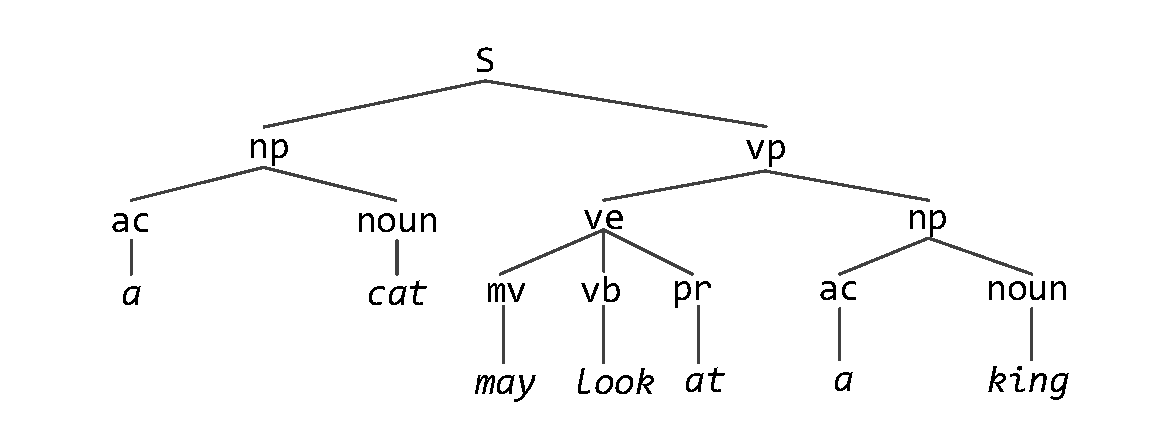
\includegraphics[scale=0.65]{gramtree}
	\end{figure}
	
\end{frame}


\begin{frame}
	\frametitle{\insertsection}
	
	\begin{itemize}
		\item A string of non-terminal symbols (words) is \textbf{grammatically correct} according to our grammar if we can build a parse tree for it. Having a grammar like one above we can
		implement \textbf{a recognizer}~--- a program that correctly classifies strings as being grammatical or not.
		\item In addition to knowing whether a string is grammatical or not, we are interested in why it is grammatical. More precisely, we often want to know what its structure is, and this is exactly the information a parse tree gives us. This kind of information would be important if we were using this sentence in some application and needed to say what it actually meant.
		A program that correctly answers if a string is grammatical and also builds a parse tree is called \textbf{a parser}.
	\end{itemize}
\end{frame}


\begin{frame}
	\frametitle{\insertsection}
	
	\begin{itemize}
		\item A context free language is a language that can be generated by a context free grammar.
		\item It is proved that some natural languages are context free (for example English and French).
		\item Many programming languages are context free languages.
		\item For this reason context free grammars are often used in compiler development.
	\end{itemize}
\end{frame}


\section{DCG in Prolog}

\begin{frame}
	\frametitle{\insertsection}
	
	Let us put it in practice.
	
	\texttt{\begin{tabular}{l}
			sentense(S) :- nounPhrase(NP), verbPhrase(VP), append(NP,VP,S).\\
			nounPhrase(NP) :- article(A), noun(N), append(A,N,NP).\\
			verbPhrase(VP) :- verbExpr(VE), nounPhrase(NP), append(VE,NP,VP).\\
			verbExpr(VE) :- modalVerb(MV),verb(V),prep(P),append([MV,V,P],VE).\\
			article([A]) :- lexicon(''article'', A).\\
			noun([N]) :- lexicon(''noun'',N).\\
			modalVerb([MV]) :- lexicon(''modal verb'',MV).\\
			verb([V]) :- lexicon(''verb'',V).\\
			prep([P]) :- lexicon(''prep'',P).
	\end{tabular}}
\end{frame}


\begin{frame}
	\frametitle{\insertsection}
	
	Predicate \texttt{lexicon/2} is used to define an alphabet (a set of terminal symbols).
	
	\texttt{\begin{tabular}{l}
			lexicon(''article``,''a``).\\
			lexicon(''article``,''the``).\\
			lexicon(''noun``,''cat``).\\
			lexicon(''noun``,''king``).\\
			lexicon(''verb``,''look``).\\
			lexicon(''modal verb``,''may``).\\
			lexicon(''prep``,''at``).
	\end{tabular}}
\end{frame}


\begin{frame}
	\frametitle{\insertsection}
	
	Then add two predicates that are handy when you start a program. Predicate \texttt{recognize} asks user to input string and starts recognizer, \texttt{generate} starts language generator that returns all phrases that are grammatically correct according to grammar.
	
	\texttt{\begin{itemize}
			\item[] recognize :- write(''Enter the phrase: ''),\\
			\quad\quad\quad\quad\quad\quad\quad current\_input(In),\\
			\quad\quad\quad\quad\quad\quad\quad read\_string(In, ''\textbackslash n'', ''\textbackslash r\textbackslash t'', \_, Phrase),\\
			\quad\quad\quad\quad\quad\quad\quad split\_string(Phrase,~''~'',~"''',~ListPhrase),\\
			\quad\quad\quad\quad\quad\quad\quad sentense(ListPhrase),!.
			\item[] generate :- sentense(Phrase),\\
			\quad\quad\quad\quad\quad\quad\quad atomics\_to\_string(Phrase,'~',String),\\
			\quad\quad\quad\quad\quad\quad\quad write(String).
	\end{itemize}}
\end{frame}


\begin{frame}
	\frametitle{\insertsection}
	
	This program works, but it is not effective.
	
	\begin{itemize}
		\item The program tries to "guess" parts of a phrase and then afterwards checks whether these can be combined to form the sentence.		
		\item Posing a query \texttt{sentense([''a'',''cat'',''may'',''look'',''at'',''a'',''king''])} will cause the program to check all possible sentences until one of them match the required one.
		\item The problem obviously is, that the goals are called with uninstantiated variables as arguments.
	\end{itemize}
\end{frame}


\begin{frame}
	\frametitle{\insertsection}
	
	We could try and solve the third problem by changing the rules in such a way that \texttt{append} becomes the first goal, but still our program would remain highly ineffective. 
	
	More to it, if we place \texttt{append} to the front generation rules will break.
	
	\texttt{\begin{tabular}{l}
			sentense(S) :- append(NP,VP,S), nounPhrase(NP), verbPhrase(VP).\\
			nounPhrase(NP) :- append(A,N,NP), article(A), noun(N).\\
			verbPhrase(VP) :- append(VE,NP,VP), verbExpr(VE), nounPhrase(NP).\\
			verbExpr(VE) :- append([MV,V,P],VE),\\
			\quad\quad\quad\quad\quad\quad\quad\quad modalVerb(MV),\\
			\quad\quad\quad\quad\quad\quad\quad\quad verb(V),\\
			\quad\quad\quad\quad\quad\quad\quad\quad prep(P).
	\end{tabular}}
\end{frame}


\section{Recognition using difference lists}


\begin{frame}
	\frametitle{\insertsection}
	
	Consider:
	
	\begin{tabular}{m{7cm} m{6cm}}
			\texttt{Ls = [x, y, z| Rs]}. & \% \texttt{Ls} is a partial list, because \texttt{Rs} is uninstantiated \\
			\uncover<2->{
				 \textbf{Symbolically}: \(Ls = [x, y, z] + Rs\) & \(\Leftrightarrow \) \texttt{append([x, y, z], Rs, Ls)} \\
			 }
			\uncover<3->{\textbf{Symbolically}: \(Ls - Rs = [x, y, z]\) & \texttt{[x, y, z]} is the \textbf{list difference} between \texttt{Ls} and \texttt{Rs} \\}
			\uncover<4->{\texttt{Rs = [].} & \texttt{Ls = [x, y, z]} \\}
			\uncover<4->{\texttt{Rs = [a, b]} & \texttt{Ls = [x, y, z, a, b]} \\}
			\uncover<5->{\texttt{Ls0 = [x, y| Ls1], Ls1 = [z, k| Ls2], Ls2 = [...| Ls3]} & An efficient concatenation \\}
			\uncover<6->{\(D_0 = Ls0 - Ls1, D_1 = Ls1 - Ls2, D_2 = Ls2 = Ls3 \) & \(D_0 + D_1 + D_2 = Ls0 - Ls3 \)}
	\end{tabular}
\end{frame}


\begin{frame}
	\frametitle{\insertsection}
	
	The pair of lists \texttt{S} and \texttt{D} represents a sentence if \((a) \) We can consume \texttt{S} and leave behind a \texttt{VP}, and the pair \texttt{S} and \texttt{VP} represents a noun phrase, and	\((b) \) We can then go on to consume \texttt{VP} leaving \texttt{D} behind, and the pair \texttt{VP, D} represents a verb phrase.
	That is: the sentence we are interested in is the difference between the contents of the two lists.
	
	\texttt{\begin{tabular}{l}
			sentense(S,D) :- nounPhrase(S,VP), verbPhrase(VP,D).\\
			nounPhrase(NP,D) :- article(NP,N), noun(N,D).\\
			verbPhrase(VP,D) :- verbExpr(VP,VE), nounPhrase(VE,D).\\
			verbExpr(VE,D) :- modalVerb(VE,MV), verb(MV,V), prep(V,D).\\
			article([A|D],D) :- lexicon(''article'',A).\\
			noun([N|D],D) :- lexicon(''noun'',N).\\
			modalVerb([MV|D],D) :- lexicon(''modal verb'',MV).\\
			verb([V|D],D) :- lexicon(''verb'',V).\\
			prep([P|D],D) :- lexicon(''prep'',P).\\
	\end{tabular}}
\end{frame}


\begin{frame}
	\frametitle{\insertsection}
	
	DCGs are really ``syntactic sugar'' for grammars written in terms of difference lists.
	
	\texttt{\begin{tabular}{l}
			sentense -{}-\textgreater~nounPhrase, verbPhrase.\\
			nounPhrase -{}-\textgreater~article, noun.\\
			verbPhrase -{}-\textgreater~verbExpr, nounPhrase.\\
			verbExpr -{}-\textgreater~modalVerb, verb, prep.\\
			article -{}-\textgreater~[''a''].\\
			article -{}-\textgreater~[''the''].\\
			noun -{}-\textgreater~[''cat''].\\
			noun -{}-\textgreater~[''king''].\\
			modalVerb -{}-\textgreater~[''may''].\\
			verb -{}-\textgreater~[''look''].\\
			prep -{}-\textgreater~[''at''].\\
	\end{tabular}}
\end{frame}


\section{Recursive rules}


\begin{frame}
	\frametitle{\insertsection}
	
	Suppose we want to add a conjunctive rule to our little grammar:
	
	\begin{table}
		\centering
		\begin{tabular}{ l }
			\rowcolor{LightGray} sentense \(\rightarrow \) sentense conjunction sentense \\
			\rowcolor{LightGray} conjunction \(\rightarrow \) and \\
			\rowcolor{LightGray} conjunction \(\rightarrow \) or \\
			\rowcolor{LightGray} conjunction \(\rightarrow \) but \\
		\end{tabular}
	\end{table}
\end{frame}


\begin{frame}
	\frametitle{\insertsection}
	
	A piece of cake, isn't it?
	
	\texttt{\begin{tabular}{l}
			sentense -{}-\textgreater~sentense, conjunction, sentense.\\
			conjunction -{}-\textgreater~[''and''].\\
			conjunction -{}-\textgreater~[''or''].\\
			conjunction -{}-\textgreater~[''but''].\\
	\end{tabular}}

	Nice try, but no...
\end{frame}


\begin{frame}
	\frametitle{\insertsection}
	
	If we place the recursive rule before the non-recursive rule
	
	\texttt{sentense -{}-\textgreater~nounPhrase, verbPhrase}
	
	then the knowledge base will contain the following two Prolog rules, in this order:
	
	\texttt{\begin{table}
			\centering
			\begin{tabular}{l}
				sentence(A, B) :- sentence(A, C), conjunction(C, D), sentence(D, B).\\
				sentence(A, B) :- nounPhrase(A, C), verbPhrase(C, B).
			\end{tabular}
	\end{table}}

	When Prolog tries to use the first rule, it immediately encounters the recursive goal, which it then tries to satisfy using the first rule, whereupon it immediately encounters the same goal and so on infinitely... Prolog goes into infinite loop and does no useful work.
	
\end{frame}


\begin{frame}
	\frametitle{\insertsection}
	
	So, let us add the recursive rule at the end of the knowledge base making Prolog always encounter the non-recursive rule first. 
	
	What happens now when we try to recognize grammatically correct sentence? Prolog seems to be able to handle it and gives the right answer. But when we pose an ungrammatical sentence, Prolog again gets into an infinite loop. 
	
	Since it is unable to recognize our sentence as consisting of a noun phrase and a verb phrase, Prolog tries to analyze it with a recursive rule again and again, and ends up in the same loop as before.
	
	\texttt{
			\begin{tabular}{l l}
				?- sentence(["a", "cat", "may", "look", "at", "the", "king"], []) & true.\\
				?- sentence(["a", "cat"], []). & ERROR
			\end{tabular}
	}
	
\end{frame}


\begin{frame}
	\frametitle{\insertsection}
	
	Recall, that in the case of ordinary recursive rule (not DCG) the trick was to change goals of the recursive rule so that the recursive goal is not the first one in the body of the rule.
	
	In the case of DCG this is not a solution, since the order of the goals determines the order of the words in the sentence.
	
	\texttt{\begin{tabular}{m{15cm}}
			sentence(A, B) :- sentence(A, C), conjunction(C, D), sentence(D, B). \(\nLeftrightarrow \) sentence(A, B) :- conjunction(C, D), sentence(A, C), sentence(D, B).
	\end{tabular}}
	
\end{frame}


\begin{frame}
	\frametitle{\insertsection}
	
	What do we do then? The only possible solution we have is to introduce new non-terminal symbols.
	
	\texttt{\begin{table}
			\centering
			\begin{tabular}{l}
				plainSentense -{}-\textgreater~nounPhrase, verbPhrase.\\
				sentense -{}-\textgreater~plainSentense.\\
				sentense -{}-\textgreater~plainSentense, conjunction, sentense.\\
			\end{tabular}
	\end{table}}
	
\end{frame}


\section{Formal languages}

\begin{frame}
	\frametitle{\insertsection}
	
	A simple example of a formal language is \(a^nb^n\). There are only two ''words`` in this language: the symbol \(a\) and the symbol \(b\).
	The language \(a^nb^n\) consist of all strings made up from these two symbols that have the following form: the string must consist of an unbroken block of \(a\)s of length \(n\), followed by an unbroken block of \(b\)s of length \(n\), and nothing else. Note that the empty word \(\mathcal{E} \) also belongs to \(a^nb^n \).
	
	\uncover<2->{\texttt{\begin{table}
				\centering
				\begin{tabular}{l}
					s --> [].\\
					s --> [a],s,[b].
				\end{tabular}
	\end{table}}}
	
\end{frame}

